
%(BEGIN_QUESTION)
% Copyright 2006, Tony R. Kuphaldt, released under the Creative Commons Attribution License (v 1.0)
% This means you may do almost anything with this work of mine, so long as you give me proper credit

A free-floating piston inside a hydraulic cylinder has a 1000 PSI of fluid pressure applied to one side of the piston, and 850 PSI of pressure applied to the other side of the piston.  The piston itself is 2.75 inches in diameter.  How much force will act on the piston, with these pressures applied to it?

$$\includegraphics[width=15.5cm]{i00155x01.eps}$$

\underbar{file i00155}
%(END_QUESTION)





%(BEGIN_ANSWER)

Net piston force = 890.936 pounds.

\vskip 10pt

In this scenario, there are two pressures fighting against each other: the 850 PSI pressure is pressing downward on the piston while the 1000 PSI pressure is pressing upward.  The resultant (differential) pressure is 150 PSI (1000 PSI - 850 PSI).  This is the pressure figure to be used in the final force calculation.

%(END_ANSWER)





%(BEGIN_NOTES)

%INDEX% Physics, fluids: pressure, force, and area

%(END_NOTES)


